\topic{Wave Equation Solutions}
%
\begin{itemize}
  \item $u_{tt} = c^2 u_{xx}$
  \item $x \in (-\infty, \infty), t \in [0, \infty)$
  \item $u(x, 0) = f(x)$
  \item $u_t(x, 0) = g(x)$
  \item $\displaystyle u(x, t) = \frac{1}{2} \left[ f(x + ct) + f(x - ct) \right] + \frac{1}{2c} \int^{x + ct}_{x - ct} g(y) \text{ dy}$
\end{itemize}
%
\begin{enumerate}
  \item Conservation of Energy
  %
  \begin{align}
    \frac{dE}{dt} & = 0
  \end{align}

  Here, let us consider the energy as:
  %
  \begin{align}
    E & = \frac{1}{2} \int^\infty_{-\infty} (u^2_t + c^2 u^2_x) \text{ dx}
  \end{align}

  Here, the first term is kinetic energy and the second term is the potential energy. Let us derive our $E$:
  %
  \begin{align}
    \frac{dE}{dt}
    & = \frac{d}{dt} \frac{1}{2} \int^\infty_{-\infty} (u^2_t + c^2 u^2_x) \text{ dx}\\
    & = \frac{1}{2} \int^\infty_{-\infty} 2u_t u_{tt} + 2 c^2 u_x u_{xt} \text{ dx}\\
    & = \int^\infty_{-\infty} u_t u_{tt} + c^2 u_x u_{xt} \text{ dx}\\
    & = \int^\infty_{-\infty} u_t c^2 u_{xx} + c^2 u_x u_{xt} \text{ dx}\\
    & = c^2 \int^\infty_{-\infty} u_t u_{xx} + u_x u_{xt} \text{ dx}
  \end{align}

  Here, let us integrate $u_{xx}$ and differentiate $u_t$:
  %
  \begin{align}
    c^2
    \left[
     u_t u_x \Big|^\infty_{-\infty} + \int^\infty_{-\infty} - u_{tx} u_x + u_x u_{xt} \text{ dx}
    \right]
    & = 0
  \end{align}

  Here, this shows our conservation of energy.
  %
  \item \topic{Domain of Dependence / Range of Influence}

  How does the solution at a point depend on the initial condition?
  % Image

  The domain of dependence is the interval between these two points:
  %
  \begin{align}
    [x_0 - ct_0, x_0 + ct_0]
  \end{align}

  If we change the initial condition of a point, where will $u$ be altered?

  The range of influence of the initial condition at point $x_0$ is
  %
  \begin{align}
    \left\{ (x, t) : \frac{| x - x_0|}{t} \leq c \right\}
  \end{align}
  %
  \item Parallelogram Property (Also valid on $x \in [a, b]$).
  %
  % Image
  %     D -1/c Slope
  %       C
  %  B    1/c Slope
  %   A
  %
  \begin{center}
    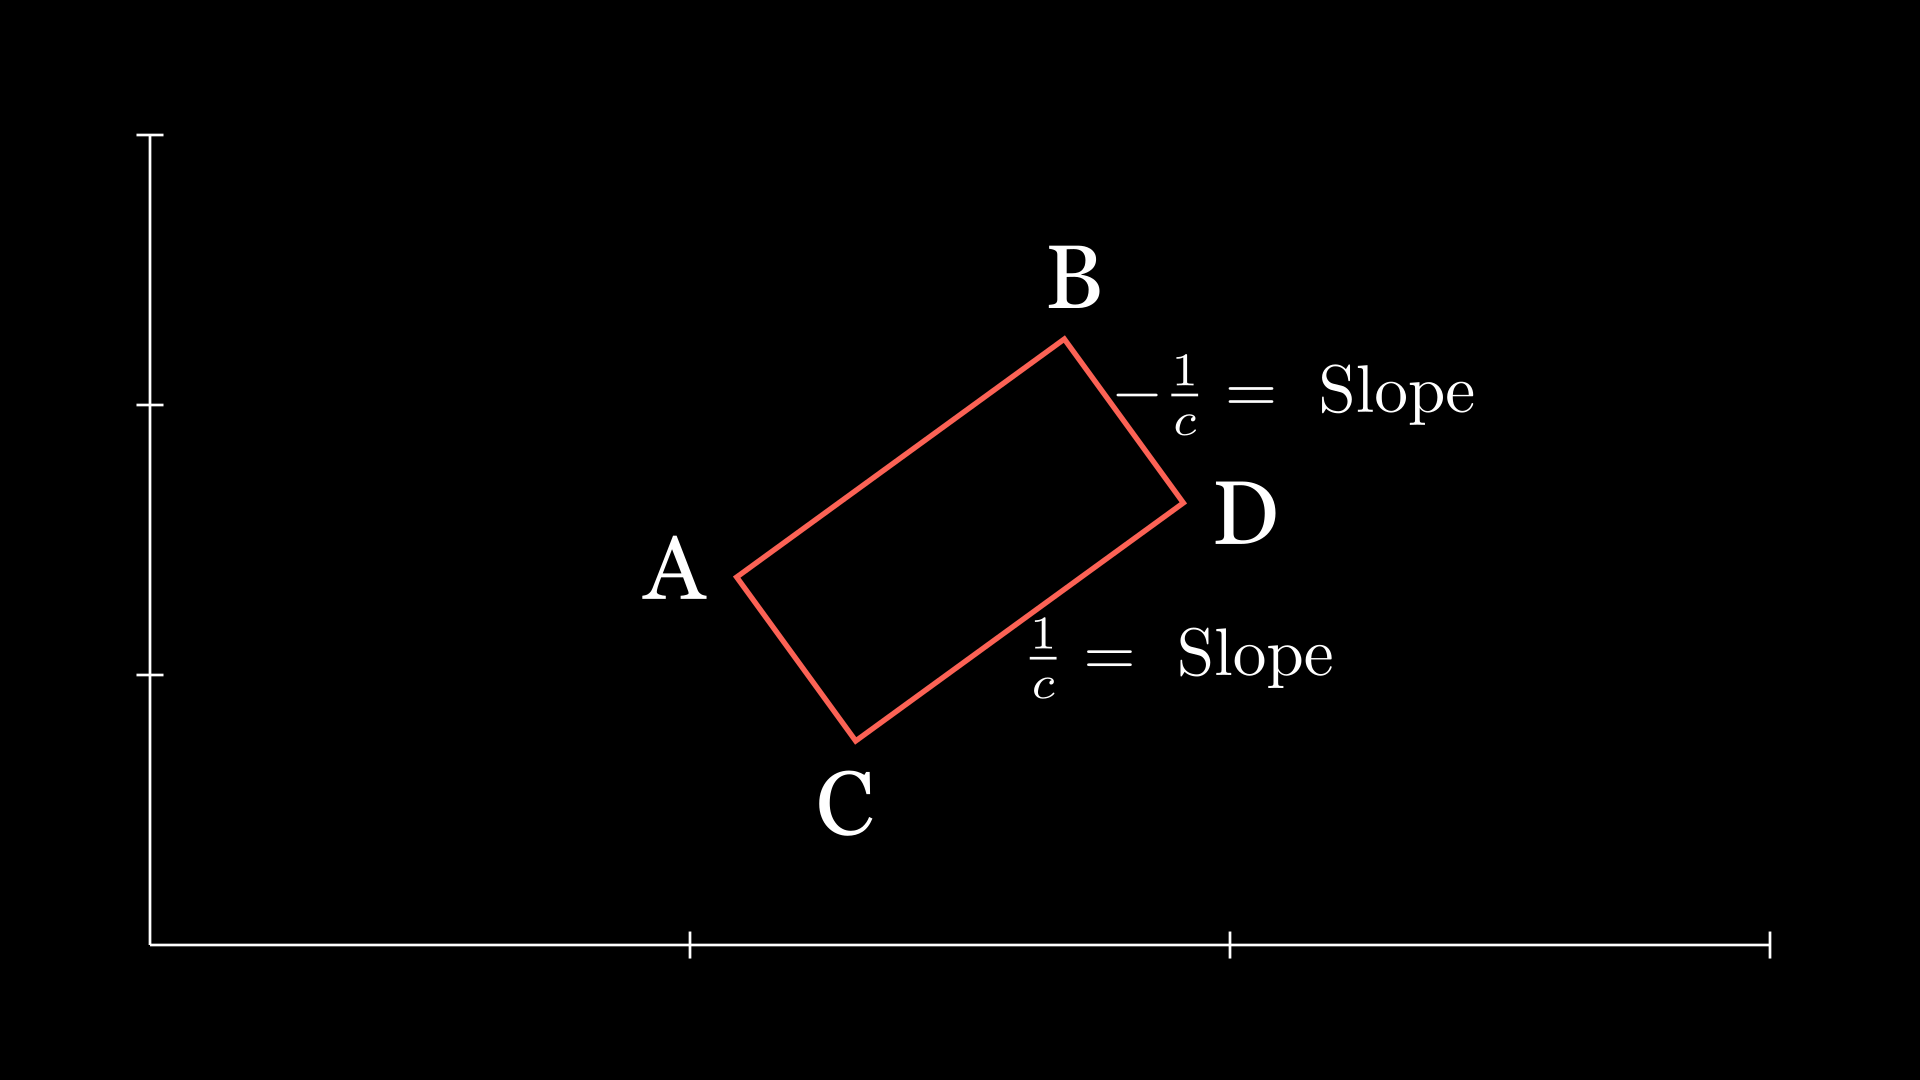
\includegraphics[height = 4cm]{Heat Equation Solution Rectangle}
  \end{center}
  \begin{align}
    u(A) + u(D) & = u(B) + u(C)
  \end{align}

  \item Reversal of Time

  You can solve the wave equation in backward time
  %
  \begin{enumerate}
    \item $x \in (-\infty, \infty)$
    \item $x \in [a, b]$
    \item $x \in \Omega \subseteq \R^n$
  \end{enumerate}

  \item Expanding to Multi-Dimensions

  We cannot expand D'Alembert's Formula in any way to $x \in \R^n, n \leq 2$.

  There are formulas for solving the wave equation for $n \leq 2$.

  The wave equation and the transport equation are both called hyperbolic equations because characteristics are involved in the solution of both.

  Here, let us write:
  %
  \begin{center}
    \begin{tabular}{l|l}
      Transport & $x + ct$\\
      Wave & $x + ct, x - ct$
    \end{tabular}\\
    \smallbreak
    \begin{tabular}{l|ll}
      Transport & $u_t = cu_x$ & $u(x, 0) = f(x)$\\
      Wave & $U_t = CU_x$ & $U(x, 0) = F(x)$
    \end{tabular}\\
    Where $U =
    \begin{bmatrix}
      u_t\\
      u_x
    \end{bmatrix}
    $
  \end{center}

  Now, let us consider:
  %
  \begin{align}
    U_t = CU_x \Rightarrow
    \begin{bmatrix}
      u_{tt}\\
      u_{xt}
    \end{bmatrix}
    & =
    \begin{bmatrix}
      0 & c^2\\
      1 & 0
    \end{bmatrix}
    \begin{bmatrix}
      u_{tx}\\
      u_{xx}
    \end{bmatrix},\\
    U(x, 0) & =
    \begin{bmatrix}
      u_t(x, 0)\\
      u_x(x, 0)
    \end{bmatrix}
    =
    \begin{bmatrix}
      g(x)\\
      f^\prime(x)
    \end{bmatrix}
  \end{align}
\end{enumerate}
